\documentclass{standalone}
\usepackage{tikz}
\usetikzlibrary{patterns, positioning}


\begin{document}
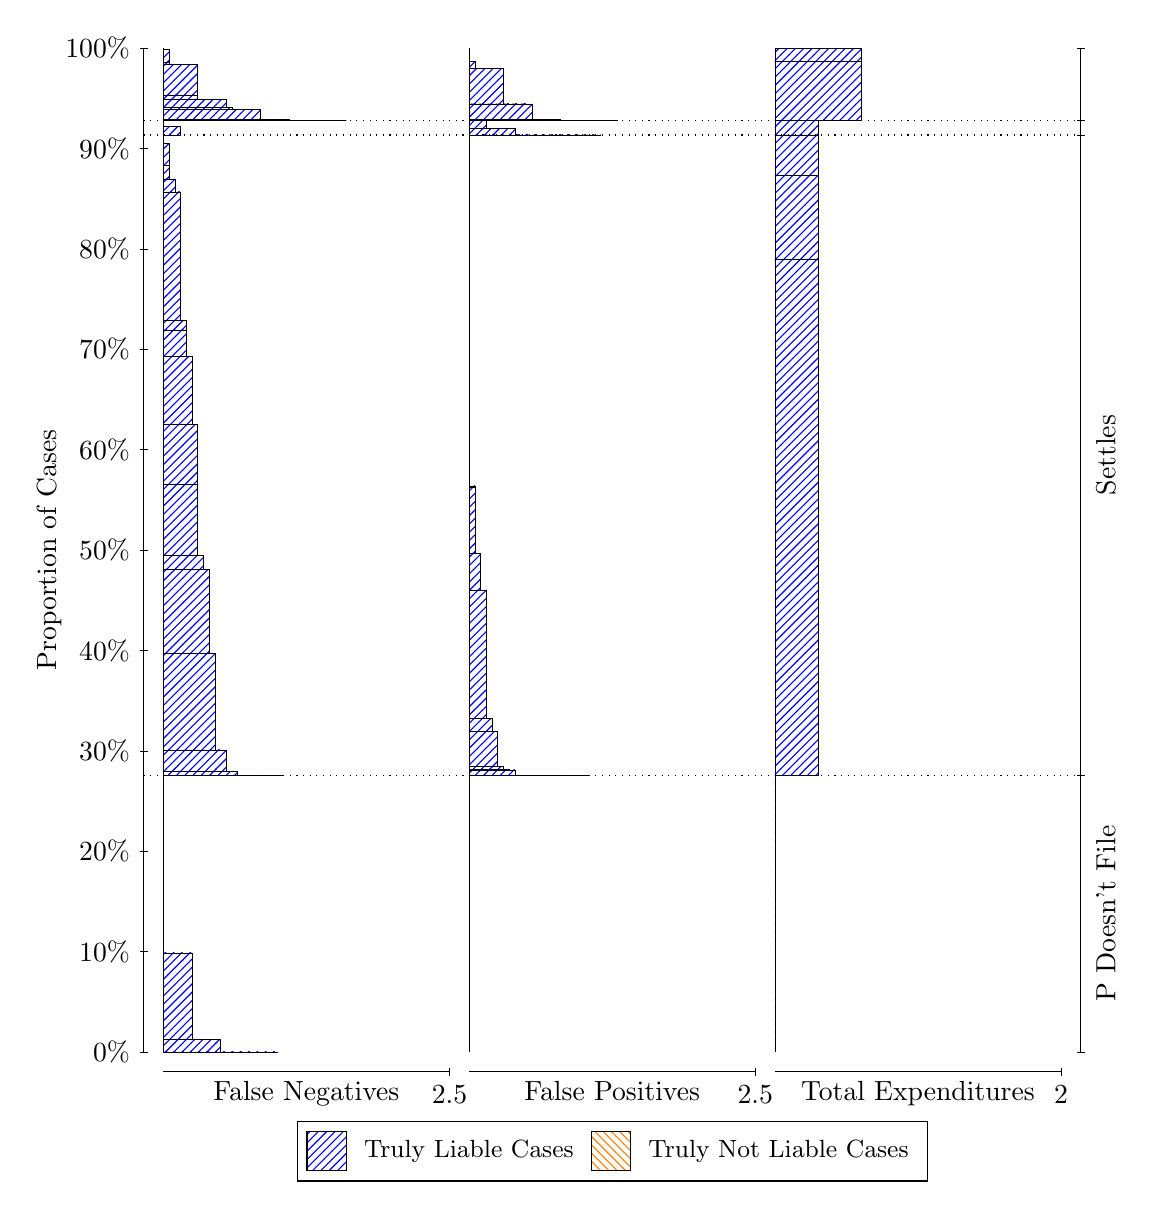
\begin{tikzpicture}
\draw[black, very thin] (1.5,1.75) -- (1.5,14.5);
\node[rotate=90, text=black, anchor=center] at (0.3, 8.125) {Proportion of Cases};
\draw[black, very thin] (1.45,1.75) -- (1.55,1.75);
\node[text=black, anchor=east] at (1.45, 1.75) {0\%};
\draw[black, very thin] (1.45,3.025) -- (1.55,3.025);
\node[text=black, anchor=east] at (1.45, 3.025) {10\%};
\draw[black, very thin] (1.45,4.3) -- (1.55,4.3);
\node[text=black, anchor=east] at (1.45, 4.3) {20\%};
\draw[black, very thin] (1.45,5.575) -- (1.55,5.575);
\node[text=black, anchor=east] at (1.45, 5.575) {30\%};
\draw[black, very thin] (1.45,6.85) -- (1.55,6.85);
\node[text=black, anchor=east] at (1.45, 6.85) {40\%};
\draw[black, very thin] (1.45,8.125) -- (1.55,8.125);
\node[text=black, anchor=east] at (1.45, 8.125) {50\%};
\draw[black, very thin] (1.45,9.4) -- (1.55,9.4);
\node[text=black, anchor=east] at (1.45, 9.4) {60\%};
\draw[black, very thin] (1.45,10.675) -- (1.55,10.675);
\node[text=black, anchor=east] at (1.45, 10.675) {70\%};
\draw[black, very thin] (1.45,11.95) -- (1.55,11.95);
\node[text=black, anchor=east] at (1.45, 11.95) {80\%};
\draw[black, very thin] (1.45,13.225) -- (1.55,13.225);
\node[text=black, anchor=east] at (1.45, 13.225) {90\%};
\draw[black, very thin] (1.45,14.5) -- (1.55,14.5);
\node[text=black, anchor=east] at (1.45, 14.5) {100\%};

\draw[black, very thin] (13.4,1.75) -- (13.4,14.5);
\draw[black, very thin] (13.35,1.75) -- (13.45,1.75);
\node[anchor=west] at (13.35, 1.75) {};
\draw[black, very thin] (13.35,5.2666) -- (13.45,5.2666);
\node[anchor=west] at (13.35, 5.2666) {};
\draw[black, very thin] (13.35,13.396) -- (13.45,13.396);
\node[anchor=west] at (13.35, 13.396) {};
\draw[black, very thin] (13.35,13.582) -- (13.45,13.582);
\node[anchor=west] at (13.35, 13.582) {};
\draw[black, very thin] (13.35,14.5) -- (13.45,14.5);
\node[anchor=west] at (13.35, 14.5) {};

\draw[black, very thin, pattern color=blue, pattern=north east lines] (1.75,1.75) rectangle (3.2033,1.75);
\draw[black, very thin, pattern color=blue, pattern=north east lines] (1.75,1.75) rectangle (2.84,1.7514);
\draw[black, very thin, pattern color=blue, pattern=north east lines] (1.75,1.7514) rectangle (2.4767,1.9141);
\draw[black, very thin, pattern color=blue, pattern=north east lines] (1.75,1.9141) rectangle (2.1133,3.0081);
\draw[black, very thin, pattern color=orange, pattern=north west lines] (1.75,3.0081) rectangle (1.75,3.0081);
\draw[black, very thin, pattern color=blue, pattern=north east lines] (1.75,3.0081) rectangle (1.75,5.2666);
\draw[black, very thin, pattern color=blue, pattern=north east lines] (1.75,5.2666) rectangle (3.276,5.2666);
\draw[black, very thin, pattern color=blue, pattern=north east lines] (1.75,5.2666) rectangle (3.1307,5.2666);
\draw[black, very thin, pattern color=blue, pattern=north east lines] (1.75,5.2666) rectangle (2.9853,5.2666);
\draw[black, very thin, pattern color=blue, pattern=north east lines] (1.75,5.2666) rectangle (2.9127,5.2666);
\draw[black, very thin, pattern color=blue, pattern=north east lines] (1.75,5.2666) rectangle (2.84,5.2666);
\draw[black, very thin, pattern color=blue, pattern=north east lines] (1.75,5.2666) rectangle (2.7673,5.2666);
\draw[black, very thin, pattern color=blue, pattern=north east lines] (1.75,5.2666) rectangle (2.6947,5.3116);
\draw[black, very thin, pattern color=blue, pattern=north east lines] (1.75,5.3116) rectangle (2.622,5.3127);
\draw[black, very thin, pattern color=blue, pattern=north east lines] (1.75,5.3127) rectangle (2.5493,5.5846);
\draw[black, very thin, pattern color=blue, pattern=north east lines] (1.75,5.5846) rectangle (2.4767,5.5855);
\draw[black, very thin, pattern color=blue, pattern=north east lines] (1.75,5.5855) rectangle (2.404,6.8103);
\draw[black, very thin, pattern color=blue, pattern=north east lines] (1.75,6.8103) rectangle (2.404,6.8168);
\draw[black, very thin, pattern color=blue, pattern=north east lines] (1.75,6.8168) rectangle (2.3313,7.8762);
\draw[black, very thin, pattern color=blue, pattern=north east lines] (1.75,7.8762) rectangle (2.2587,8.0603);
\draw[black, very thin, pattern color=blue, pattern=north east lines] (1.75,8.0603) rectangle (2.186,8.9624);
\draw[black, very thin, pattern color=blue, pattern=north east lines] (1.75,8.9624) rectangle (2.186,9.7239);
\draw[black, very thin, pattern color=blue, pattern=north east lines] (1.75,9.7239) rectangle (2.1133,10.586);
\draw[black, very thin, pattern color=blue, pattern=north east lines] (1.75,10.586) rectangle (2.0407,10.921);
\draw[black, very thin, pattern color=blue, pattern=north east lines] (1.75,10.921) rectangle (2.0407,11.044);
\draw[black, very thin, pattern color=blue, pattern=north east lines] (1.75,11.044) rectangle (1.968,12.672);
\draw[black, very thin, pattern color=blue, pattern=north east lines] (1.75,12.672) rectangle (1.8953,12.838);
\draw[black, very thin, pattern color=blue, pattern=north east lines] (1.75,12.838) rectangle (1.8227,13.008);
\draw[black, very thin, pattern color=blue, pattern=north east lines] (1.75,13.008) rectangle (1.8227,13.286);
\draw[black, very thin, pattern color=blue, pattern=north east lines] (1.75,13.286) rectangle (1.75,13.287);
\draw[black, very thin, pattern color=orange, pattern=north west lines] (1.75,13.287) rectangle (1.75,13.287);
\draw[black, very thin, pattern color=blue, pattern=north east lines] (1.75,13.287) rectangle (1.75,13.396);
\draw[black, very thin, pattern color=blue, pattern=north east lines] (1.75,13.396) rectangle (1.968,13.502);
\draw[black, very thin, pattern color=orange, pattern=north west lines] (1.75,13.502) rectangle (1.75,13.502);
\draw[black, very thin, pattern color=blue, pattern=north east lines] (1.75,13.502) rectangle (1.75,13.582);
\draw[black, very thin, pattern color=blue, pattern=north east lines] (1.75,13.582) rectangle (4.0753,13.582);
\draw[black, very thin, pattern color=blue, pattern=north east lines] (1.75,13.582) rectangle (3.712,13.582);
\draw[black, very thin, pattern color=blue, pattern=north east lines] (1.75,13.582) rectangle (3.3487,13.596);
\draw[black, very thin, pattern color=blue, pattern=north east lines] (1.75,13.596) rectangle (3.276,13.596);
\draw[black, very thin, pattern color=blue, pattern=north east lines] (1.75,13.596) rectangle (2.9853,13.722);
\draw[black, very thin, pattern color=blue, pattern=north east lines] (1.75,13.722) rectangle (2.9127,13.722);
\draw[black, very thin, pattern color=blue, pattern=north east lines] (1.75,13.722) rectangle (2.622,13.751);
\draw[black, very thin, pattern color=blue, pattern=north east lines] (1.75,13.751) rectangle (2.5493,13.845);
\draw[black, very thin, pattern color=blue, pattern=north east lines] (1.75,13.845) rectangle (2.2587,13.845);
\draw[black, very thin, pattern color=blue, pattern=north east lines] (1.75,13.845) rectangle (2.186,13.905);
\draw[black, very thin, pattern color=blue, pattern=north east lines] (1.75,13.905) rectangle (2.186,14.292);
\draw[black, very thin, pattern color=blue, pattern=north east lines] (1.75,14.292) rectangle (1.8953,14.292);
\draw[black, very thin, pattern color=blue, pattern=north east lines] (1.75,14.292) rectangle (1.8227,14.324);
\draw[black, very thin, pattern color=blue, pattern=north east lines] (1.75,14.324) rectangle (1.8227,14.484);
\draw[black, very thin, pattern color=orange, pattern=north west lines] (1.75,14.484) rectangle (1.75,14.484);
\draw[black, very thin, pattern color=blue, pattern=north east lines] (1.75,14.484) rectangle (1.75,14.5);
\draw[black, very thin, pattern color=orange, pattern=north west lines] (5.6333,1.75) rectangle (5.6333,1.75);
\draw[black, very thin, pattern color=blue, pattern=north east lines] (5.6333,1.75) rectangle (5.6333,5.2666);
\draw[black, very thin, pattern color=orange, pattern=north west lines] (5.6333,5.2666) rectangle (7.1593,5.2666);
\draw[black, very thin, pattern color=blue, pattern=north east lines] (5.6333,5.2666) rectangle (7.1593,5.2666);
\draw[black, very thin, pattern color=orange, pattern=north west lines] (5.6333,5.2666) rectangle (6.8687,5.2666);
\draw[black, very thin, pattern color=blue, pattern=north east lines] (5.6333,5.2666) rectangle (6.8687,5.2666);
\draw[black, very thin, pattern color=blue, pattern=north east lines] (5.6333,5.2666) rectangle (6.796,5.2666);
\draw[black, very thin, pattern color=orange, pattern=north west lines] (5.6333,5.2666) rectangle (6.7233,5.2666);
\draw[black, very thin, pattern color=blue, pattern=north east lines] (5.6333,5.2666) rectangle (6.7233,5.2666);
\draw[black, very thin, pattern color=orange, pattern=north west lines] (5.6333,5.2666) rectangle (6.578,5.2666);
\draw[black, very thin, pattern color=blue, pattern=north east lines] (5.6333,5.2666) rectangle (6.578,5.2666);
\draw[black, very thin, pattern color=blue, pattern=north east lines] (5.6333,5.2666) rectangle (6.5053,5.2666);
\draw[black, very thin, pattern color=blue, pattern=north east lines] (5.6333,5.2666) rectangle (6.4327,5.2666);
\draw[black, very thin, pattern color=orange, pattern=north west lines] (5.6333,5.2666) rectangle (6.4327,5.2666);
\draw[black, very thin, pattern color=blue, pattern=north east lines] (5.6333,5.2666) rectangle (6.4327,5.2666);
\draw[black, very thin, pattern color=blue, pattern=north east lines] (5.6333,5.2666) rectangle (6.36,5.2669);
\draw[black, very thin, pattern color=orange, pattern=north west lines] (5.6333,5.2669) rectangle (6.2873,5.2669);
\draw[black, very thin, pattern color=blue, pattern=north east lines] (5.6333,5.2669) rectangle (6.2873,5.2674);
\draw[black, very thin, pattern color=blue, pattern=north east lines] (5.6333,5.2674) rectangle (6.2147,5.3314);
\draw[black, very thin, pattern color=orange, pattern=north west lines] (5.6333,5.3314) rectangle (6.142,5.3314);
\draw[black, very thin, pattern color=blue, pattern=north east lines] (5.6333,5.3314) rectangle (6.142,5.3423);
\draw[black, very thin, pattern color=blue, pattern=north east lines] (5.6333,5.3423) rectangle (6.0693,5.3762);
\draw[black, very thin, pattern color=blue, pattern=north east lines] (5.6333,5.3762) rectangle (6.0693,5.3769);
\draw[black, very thin, pattern color=orange, pattern=north west lines] (5.6333,5.3769) rectangle (5.9967,5.3769);
\draw[black, very thin, pattern color=blue, pattern=north east lines] (5.6333,5.3769) rectangle (5.9967,5.8246);
\draw[black, very thin, pattern color=blue, pattern=north east lines] (5.6333,5.8246) rectangle (5.924,5.9908);
\draw[black, very thin, pattern color=blue, pattern=north east lines] (5.6333,5.9908) rectangle (5.8513,7.6191);
\draw[black, very thin, pattern color=blue, pattern=north east lines] (5.6333,7.6191) rectangle (5.7787,8.0772);
\draw[black, very thin, pattern color=blue, pattern=north east lines] (5.6333,8.0772) rectangle (5.706,8.9198);
\draw[black, very thin, pattern color=blue, pattern=north east lines] (5.6333,8.9198) rectangle (5.706,8.939);
\draw[black, very thin, pattern color=blue, pattern=north east lines] (5.6333,8.939) rectangle (5.6333,13.396);
\draw[black, very thin, pattern color=orange, pattern=north west lines] (5.6333,13.396) rectangle (7.3047,13.396);
\draw[black, very thin, pattern color=blue, pattern=north east lines] (5.6333,13.396) rectangle (7.3047,13.396);
\draw[black, very thin, pattern color=blue, pattern=north east lines] (5.6333,13.396) rectangle (6.9413,13.396);
\draw[black, very thin, pattern color=blue, pattern=north east lines] (5.6333,13.396) rectangle (6.578,13.397);
\draw[black, very thin, pattern color=blue, pattern=north east lines] (5.6333,13.397) rectangle (6.2147,13.477);
\draw[black, very thin, pattern color=blue, pattern=north east lines] (5.6333,13.477) rectangle (5.8513,13.582);
\draw[black, very thin, pattern color=orange, pattern=north west lines] (5.6333,13.582) rectangle (7.5227,13.582);
\draw[black, very thin, pattern color=blue, pattern=north east lines] (5.6333,13.582) rectangle (7.5227,13.582);
\draw[black, very thin, pattern color=orange, pattern=north west lines] (5.6333,13.582) rectangle (7.1593,13.582);
\draw[black, very thin, pattern color=blue, pattern=north east lines] (5.6333,13.582) rectangle (7.1593,13.583);
\draw[black, very thin, pattern color=orange, pattern=north west lines] (5.6333,13.583) rectangle (6.796,13.583);
\draw[black, very thin, pattern color=blue, pattern=north east lines] (5.6333,13.583) rectangle (6.796,13.598);
\draw[black, very thin, pattern color=orange, pattern=north west lines] (5.6333,13.598) rectangle (6.4327,13.598);
\draw[black, very thin, pattern color=blue, pattern=north east lines] (5.6333,13.598) rectangle (6.4327,13.791);
\draw[black, very thin, pattern color=orange, pattern=north west lines] (5.6333,13.791) rectangle (6.36,13.791);
\draw[black, very thin, pattern color=blue, pattern=north east lines] (5.6333,13.791) rectangle (6.36,13.791);
\draw[black, very thin, pattern color=blue, pattern=north east lines] (5.6333,13.791) rectangle (6.0693,14.238);
\draw[black, very thin, pattern color=orange, pattern=north west lines] (5.6333,14.238) rectangle (5.9967,14.238);
\draw[black, very thin, pattern color=blue, pattern=north east lines] (5.6333,14.238) rectangle (5.9967,14.238);
\draw[black, very thin, pattern color=blue, pattern=north east lines] (5.6333,14.238) rectangle (5.706,14.332);
\draw[black, very thin, pattern color=orange, pattern=north west lines] (5.6333,14.332) rectangle (5.6333,14.332);
\draw[black, very thin, pattern color=blue, pattern=north east lines] (5.6333,14.332) rectangle (5.6333,14.5);
\draw[black, very thin, pattern color=orange, pattern=north west lines] (9.5167,1.75) rectangle (9.5167,1.75);
\draw[black, very thin, pattern color=blue, pattern=north east lines] (9.5167,1.75) rectangle (9.5167,5.2666);
\draw[black, very thin, pattern color=orange, pattern=north west lines] (9.5167,5.2666) rectangle (10.062,5.2666);
\draw[black, very thin, pattern color=blue, pattern=north east lines] (9.5167,5.2666) rectangle (10.062,11.814);
\draw[black, very thin, pattern color=orange, pattern=north west lines] (9.5167,11.814) rectangle (10.062,11.814);
\draw[black, very thin, pattern color=blue, pattern=north east lines] (9.5167,11.814) rectangle (10.062,12.885);
\draw[black, very thin, pattern color=orange, pattern=north west lines] (9.5167,12.885) rectangle (10.062,12.885);
\draw[black, very thin, pattern color=blue, pattern=north east lines] (9.5167,12.885) rectangle (10.062,13.396);
\draw[black, very thin, pattern color=orange, pattern=north west lines] (9.5167,13.396) rectangle (10.062,13.396);
\draw[black, very thin, pattern color=blue, pattern=north east lines] (9.5167,13.396) rectangle (10.062,13.582);
\draw[black, very thin, pattern color=orange, pattern=north west lines] (9.5167,13.582) rectangle (10.607,13.582);
\draw[black, very thin, pattern color=blue, pattern=north east lines] (9.5167,13.582) rectangle (10.607,14.332);
\draw[black, very thin, pattern color=orange, pattern=north west lines] (9.5167,14.332) rectangle (10.607,14.332);
\draw[black, very thin, pattern color=blue, pattern=north east lines] (9.5167,14.332) rectangle (10.607,14.5);
\draw[black, dotted] (1.5,5.2666) -- (13.4,5.2666);
\draw[black, dotted] (1.5,13.396) -- (13.4,13.396);
\draw[black, dotted] (1.5,13.582) -- (13.4,13.582);
\draw[black, very thin] (1.75,1.5) -- (5.3833,1.5);
\node[text=black, anchor=north] at (3.5667, 1.5) {False Negatives};
\draw[black, very thin] (5.3833,1.45) -- (5.3833,1.55);
\node[text=black, anchor=north] at (5.3833, 1.45) {2.5};

\draw[black, very thin] (5.6333,1.5) -- (9.2667,1.5);
\node[text=black, anchor=north] at (7.45, 1.5) {False Positives};
\draw[black, very thin] (9.2667,1.45) -- (9.2667,1.55);
\node[text=black, anchor=north] at (9.2667, 1.45) {2.5};

\draw[black, very thin] (9.5167,1.5) -- (13.15,1.5);
\node[text=black, anchor=north] at (11.333, 1.5) {Total Expenditures};
\draw[black, very thin] (13.15,1.45) -- (13.15,1.55);
\node[text=black, anchor=north] at (13.15, 1.45) {2};

\node[text=black, centered, rotate=90] at (13.72, 3.5083) {P Doesn't File};
\node[text=black, centered, rotate=90] at (13.72, 9.3314) {Settles};



\draw (7.449999999999999,1.5) node[draw=none] (baseCoordinate) {};
\begin{scope}[align=center]
        \matrix[scale=0.5, draw=black, below=0.5cm of baseCoordinate, nodes={draw}, column sep=0.1cm]{
            \node[rectangle, draw, minimum width=0.5cm, minimum height=0.5cm, pattern color=blue, pattern=north east lines] {}; &
            \node[draw=none, font=\small, text=black] (B) {Truly Liable Cases}; &
            \node[rectangle, draw, minimum width=0.5cm, minimum height=0.5cm, pattern color=orange, pattern=north west lines] {}; &
            \node[draw=none, font=\small, text=black] (B) {Truly Not Liable Cases}; \\
            };
\end{scope}

\end{tikzpicture}
\end{document}